\documentclass[a4paper]{article}

\usepackage[utf8]{inputenc}
\usepackage{a4wide,color,Sweave,url,amsmath,booktabs,longtable,eurosym}
\newenvironment{question}{\item \textbf{Problem}\newline}{}
\newenvironment{solution}{\textbf{Solution}\newline}{}
\newenvironment{answerlist}{\renewcommand{\labelenumi}{(\alph{enumi})}\begin{enumerate}}{\end{enumerate}}
\providecommand{\tightlist}{\setlength{\itemsep}{0pt}\setlength{\parskip}{0pt}}

\setkeys{Gin}{keepaspectratio}

\begin{document}
\begin{enumerate}

\begin{question}
A continuous random variable (spinner/random number generator/infinite
population) can be visualized with a density curve, a spinner, and a
cumulative curve.

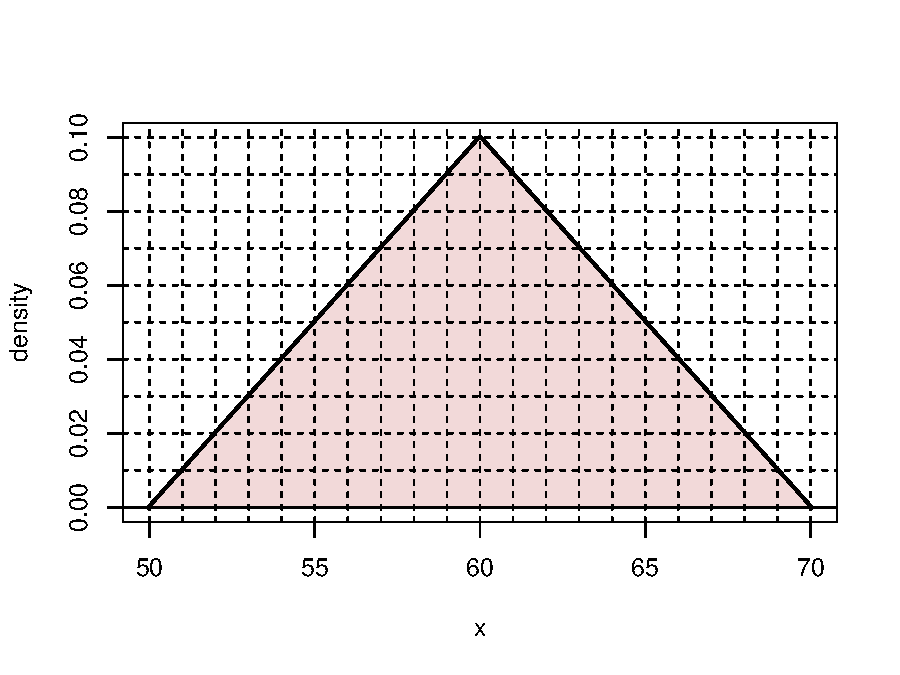
\includegraphics{unnamed-chunk-1-1.pdf}\\

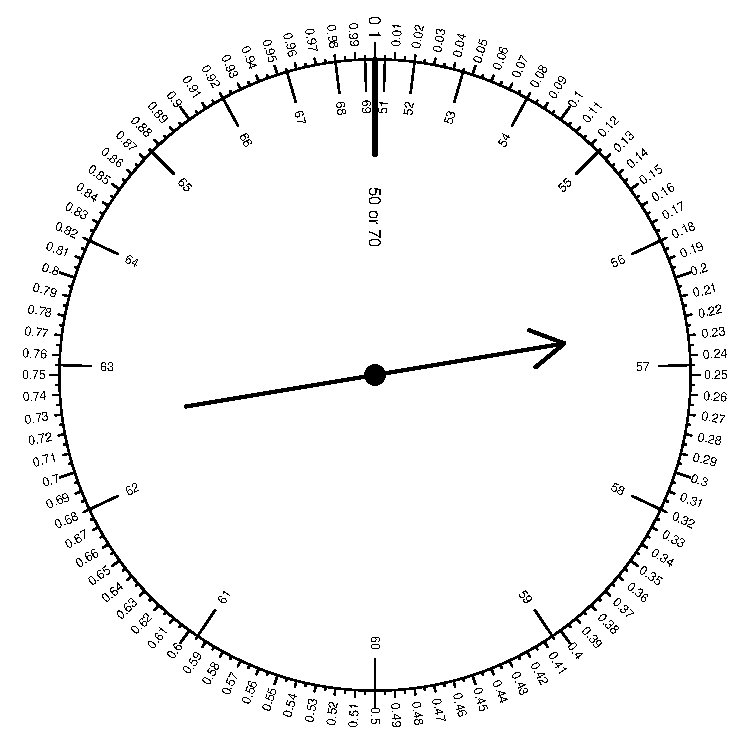
\includegraphics{unnamed-chunk-2-1.pdf}\\

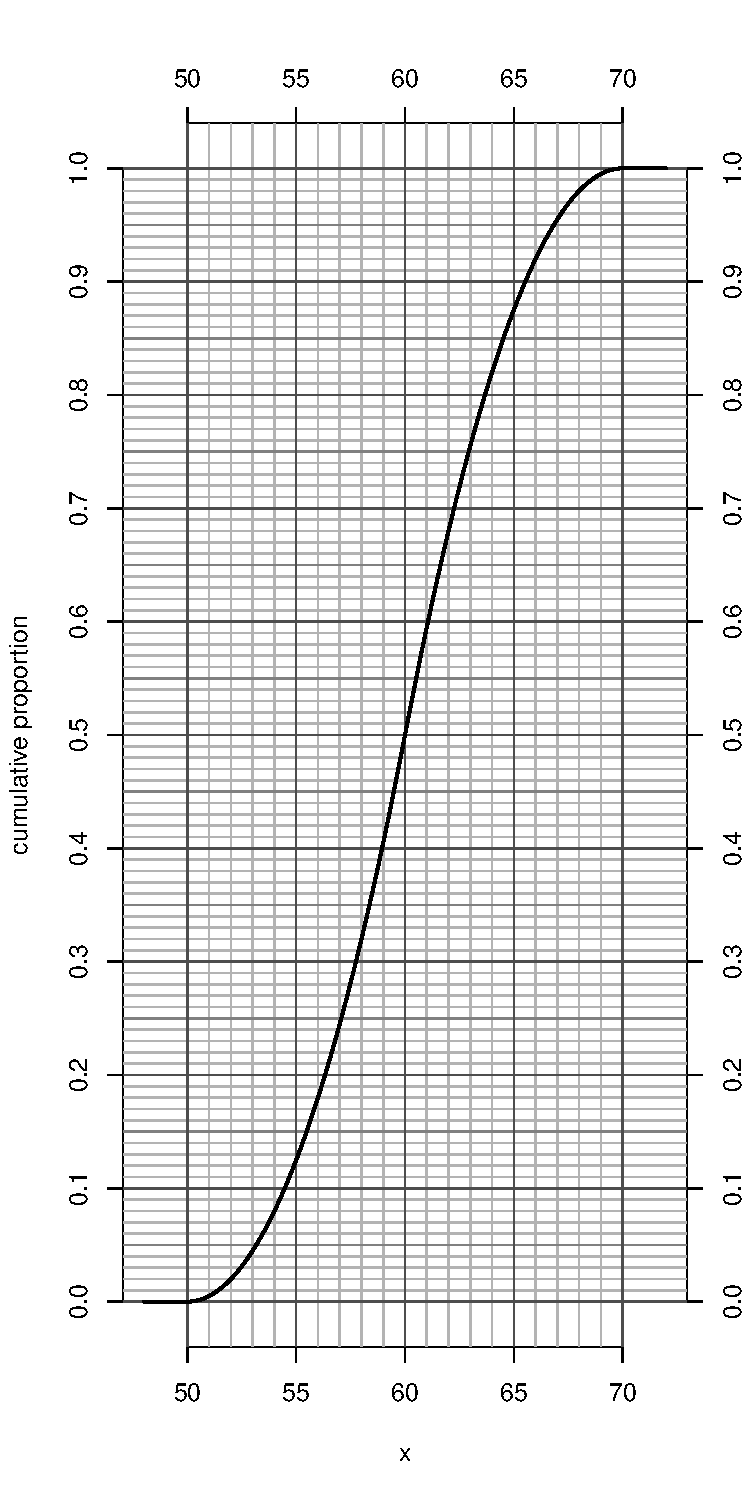
\includegraphics{unnamed-chunk-3-1.pdf}\\
\begin{answerlist}
  \item Evaluate \(\text{prop}[\mathbf{x}<68]\)
  \item Evaluate \(\text{prop}[\mathbf{x}>54]\)
  \item Evaluate \(\text{prop}[|\mathbf{x}-60|<2]\)
  \item Determine integer \(b\) such that \(\text{prop}[\mathbf{x}<b]=0.82\)
  \item Determine integer \(b\) such that \(\text{prop}[\mathbf{x}>b]=0.82\)
  \item Determine integer \(r\) such that
\(\text{prop}[|\mathbf{x}-63|<r]=0.42\)
\end{answerlist}
\end{question}

\begin{solution}
For each problem, you can use any of the visualizations. In short, the
answers:

\begin{verbatim}
## 0.98 0.92 0.36 64 56 3
\end{verbatim}
\begin{answerlist}
  \item The answer is 0.98 because \(\text{prop}[\mathbf{x}<68]=0.98\). The
following visualizations show this. The density curve can be used by
counting percent boxes. Each box adds 0.01 to the proportion. You may
need to count half boxes, or find partial boxes that add to whole boxes.
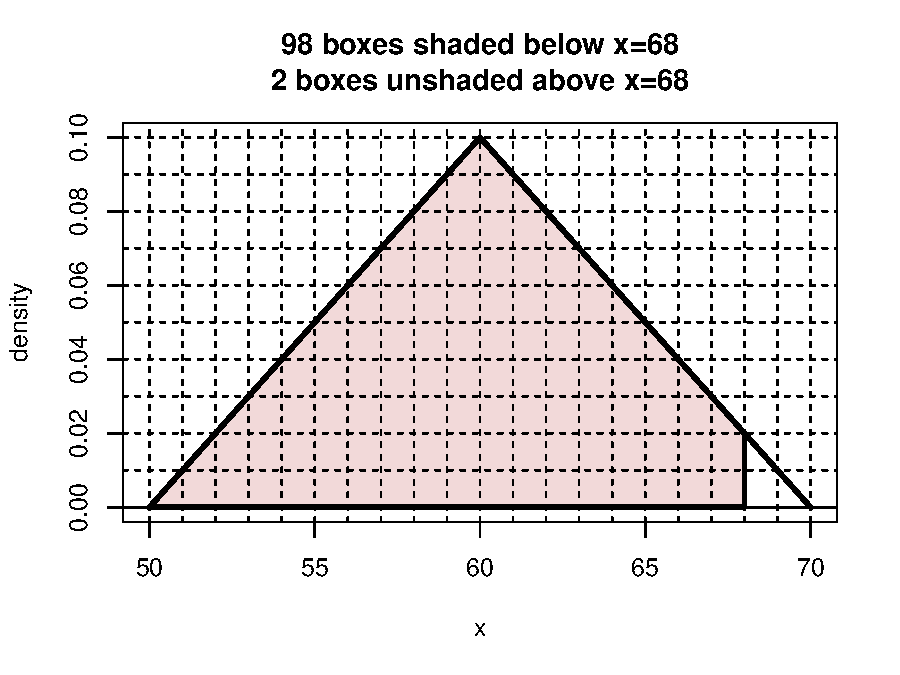
\includegraphics{unnamed-chunk-5-1.pdf} ~ On the spinner, you can
determine the size of a region by using the outside tickmarks.
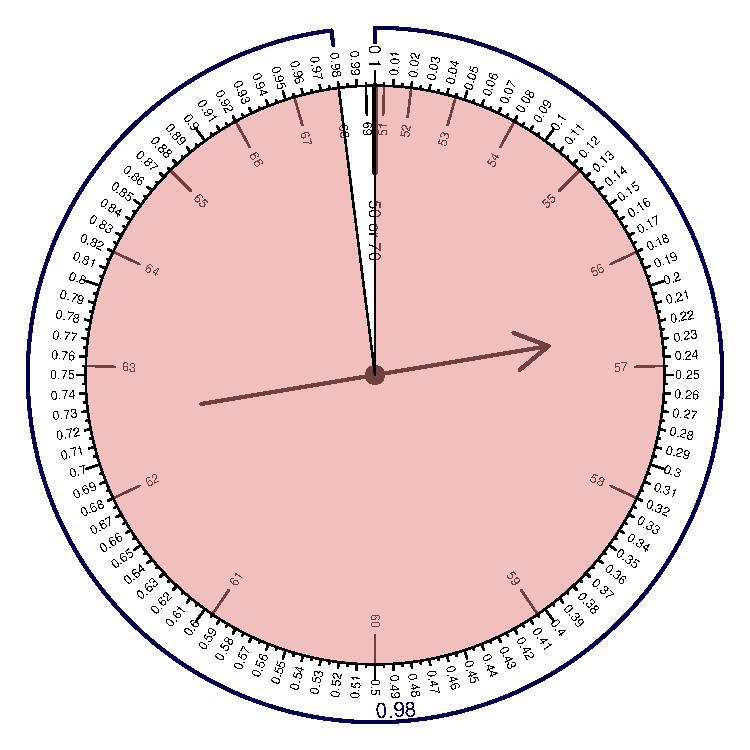
\includegraphics{unnamed-chunk-6-1.pdf} ~ You need to read coordinates
to use the cumulative curve. 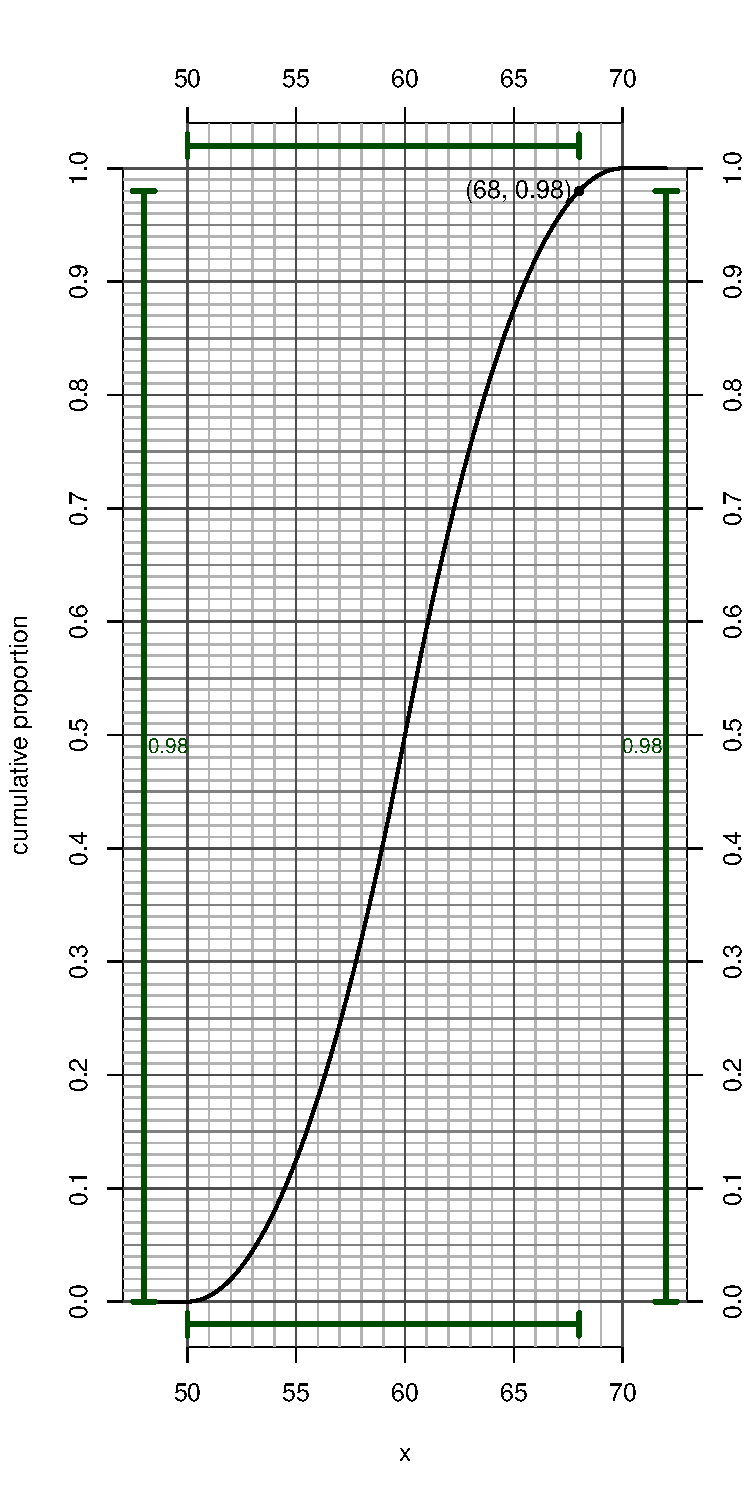
\includegraphics{unnamed-chunk-7-1.pdf} ~
  \item The answer is 0.92 because \(\text{prop}[\mathbf{x}>54]=0.92\). The
following visualizations show this. The density curve can be used by
counting percent boxes. Each box adds 0.01 to the proportion. You may
need to count half boxes, or find partial boxes that add to whole boxes.
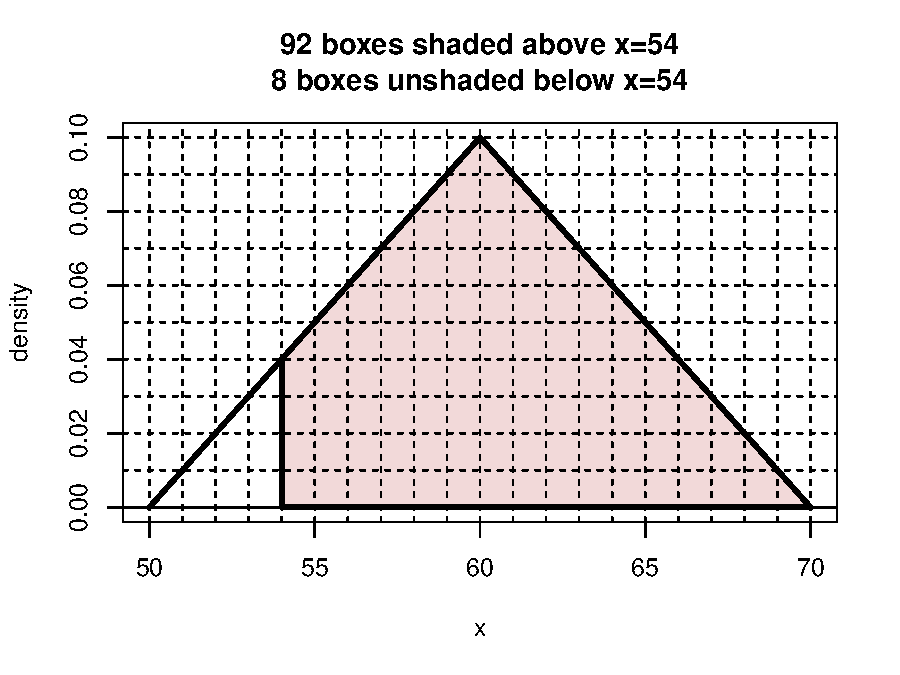
\includegraphics{unnamed-chunk-8-1.pdf} ~ On the spinner, you can
determine the size of a region by using the outside tickmarks.
\[1-0.08=0.92\] 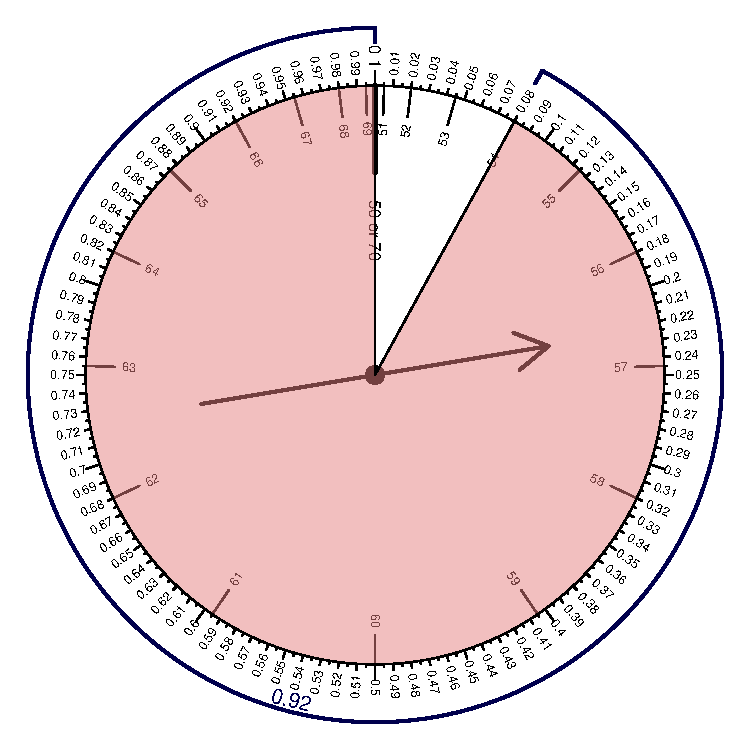
\includegraphics{unnamed-chunk-9-1.pdf} ~ You need to
read coordinates to use the cumulative curve. \[1-0.08=0.92\]
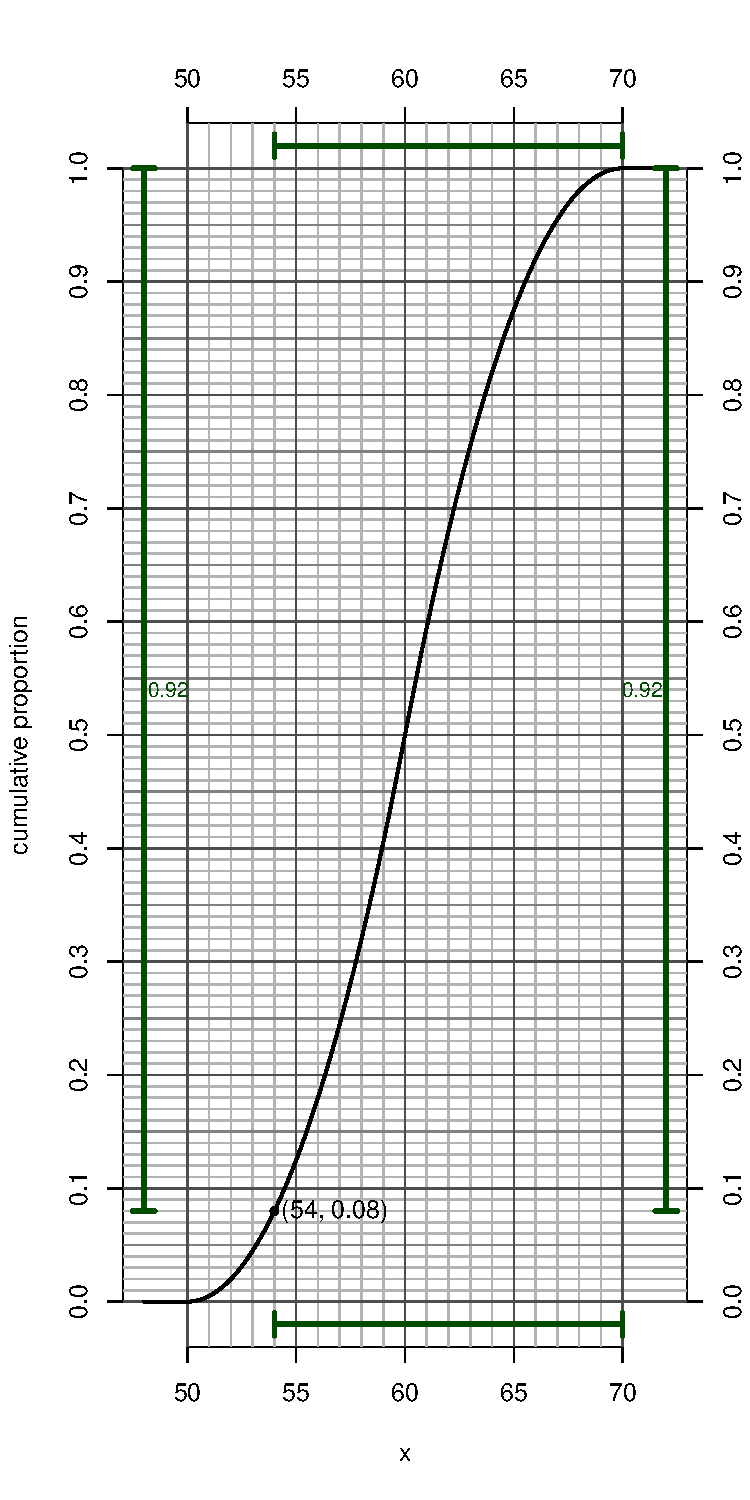
\includegraphics{unnamed-chunk-10-1.pdf} ~
  \item The answer is 0.36 because \(\text{prop}[|\mathbf{x}-60|<2]=0.36\). It
helps to point out this interval has a center of 60 and a radius of 2,
and thus a lower bound of 58 and an upper bound of 62. The following
visualizations show this. The density curve can be used by counting
percent boxes. Each box adds 0.01 to the proportion. You may need to
count half boxes, or find partial boxes that add to whole boxes.
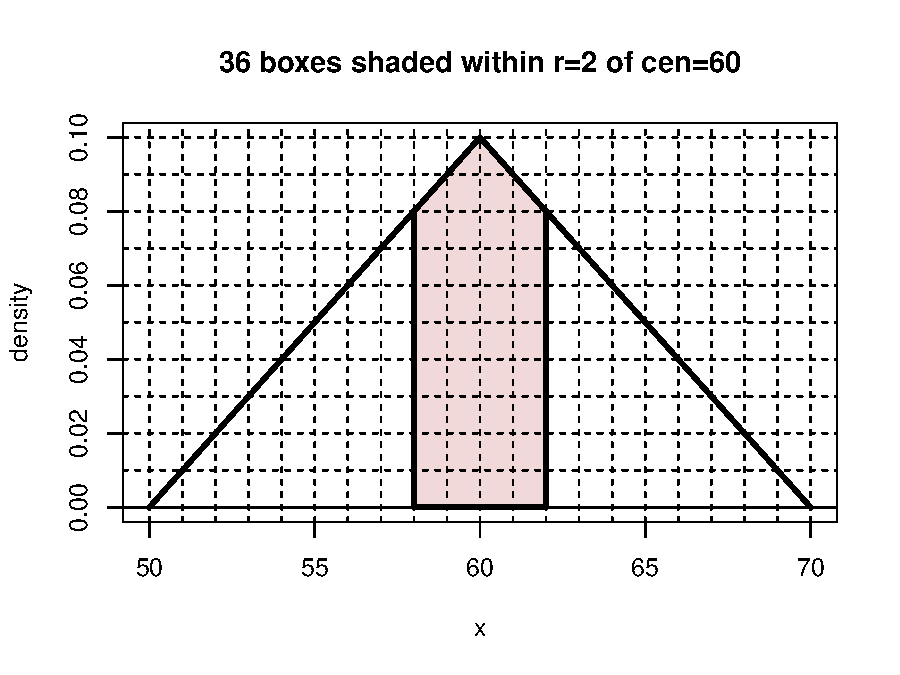
\includegraphics{unnamed-chunk-11-1.pdf} ~ On the spinner, you can
determine the size of a region by using the outside tickmarks. The lower
bound is at \(x=58\), which corresponds to a cumulative proportion of
0.32. The upper bound is at \(x=62\), which corresponds to a cumulative
proportion of 0.68. \[0.68-0.32=0.36\]
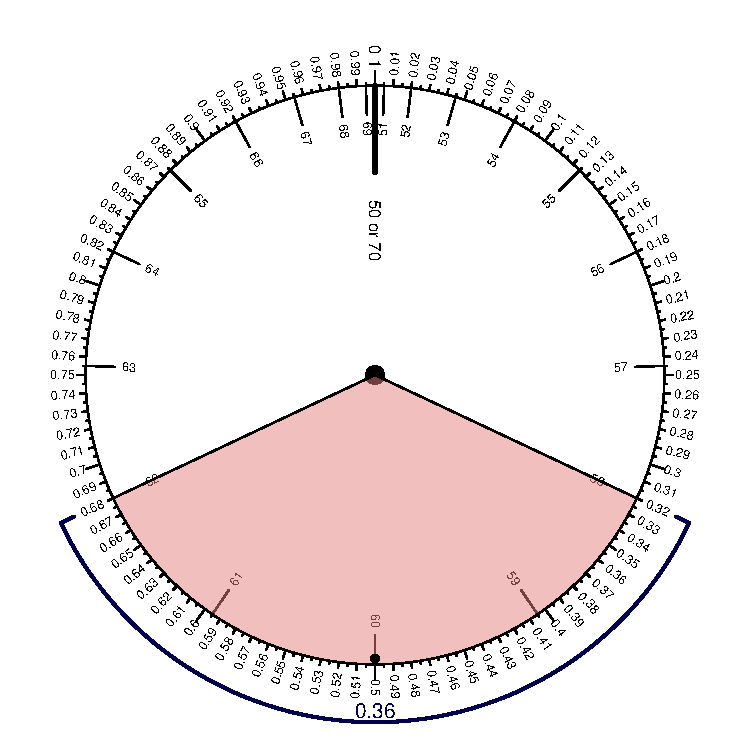
\includegraphics{unnamed-chunk-12-1.pdf} ~ You need to read coordinates
to use the cumulative curve. The lower bound is at \(x=58\), which
corresponds to a cumulative proportion of 0.32. The upper bound is at
\(x=62\), which corresponds to a cumulative proportion of 0.68.
\[0.68-0.32=0.36\] 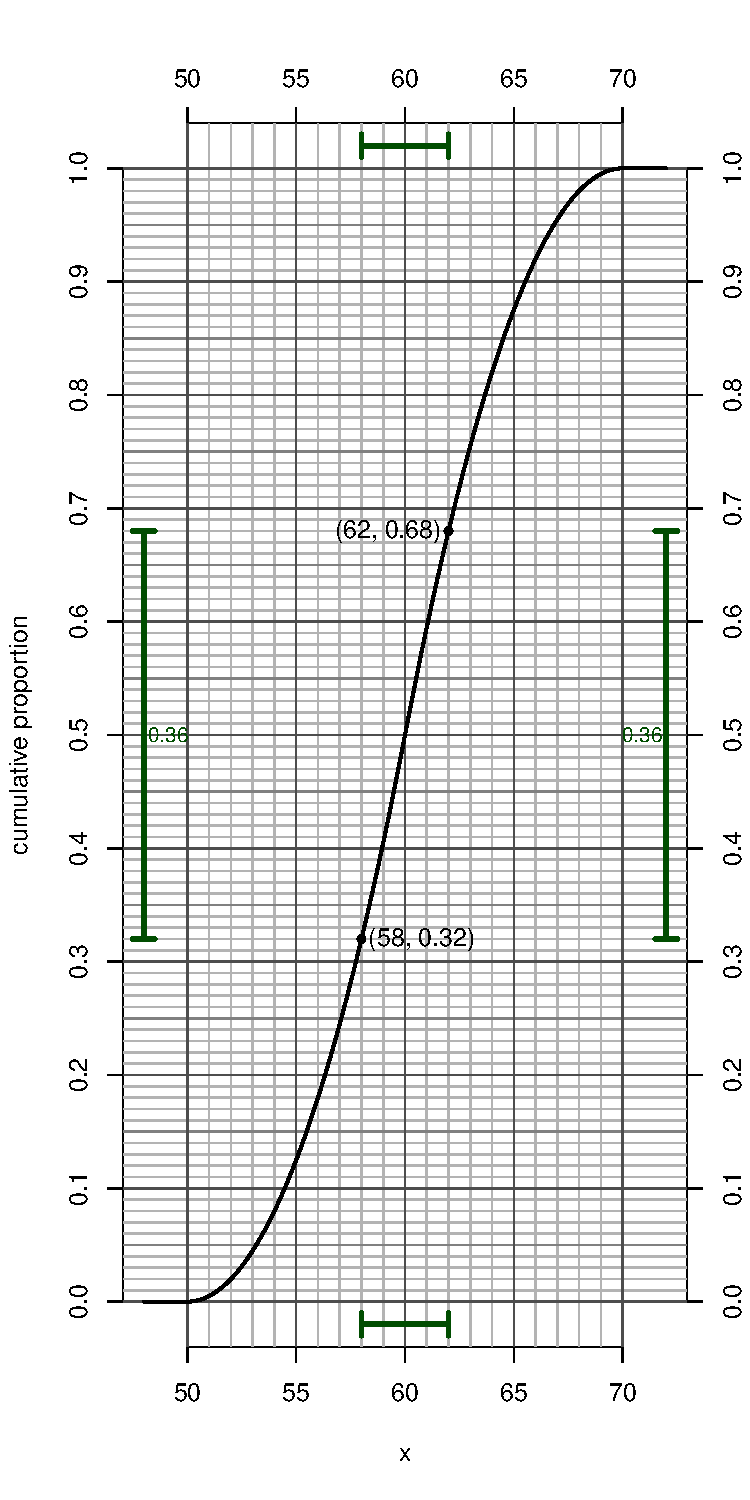
\includegraphics{unnamed-chunk-13-1.pdf} ~
  \item The answer is 64 because \(\text{prop}[\mathbf{x}<64]=0.82\). The
following visualizations show this. The density curve can be used by
counting percent boxes. Each box adds 0.01 to the proportion. You may
need to count half boxes, or find partial boxes that add to whole boxes.
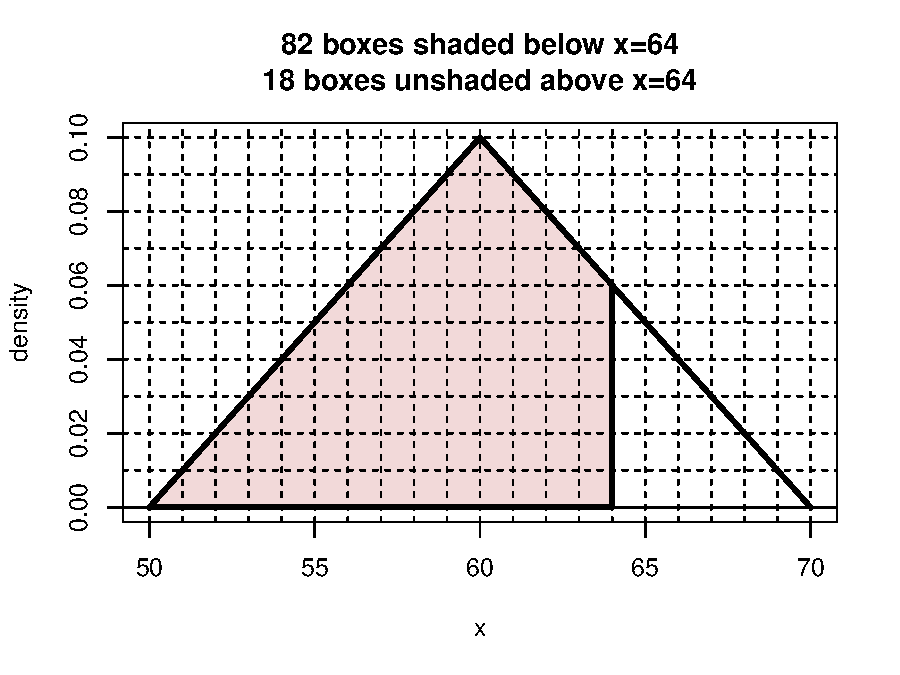
\includegraphics{unnamed-chunk-14-1.pdf} ~ On the spinner, you can
determine the size of a region by using the outside tickmarks.
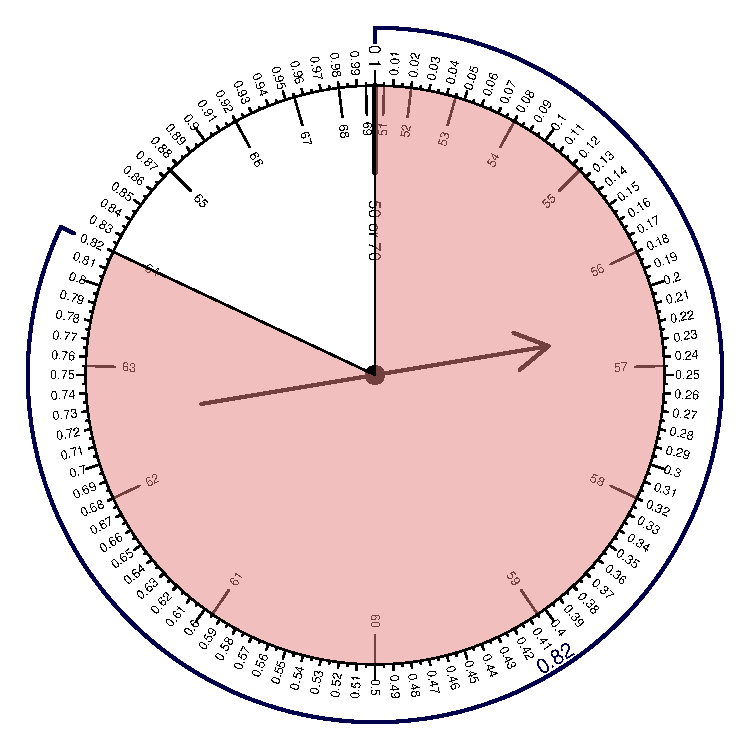
\includegraphics{unnamed-chunk-15-1.pdf} ~ You need to read coordinates
to use the cumulative curve. 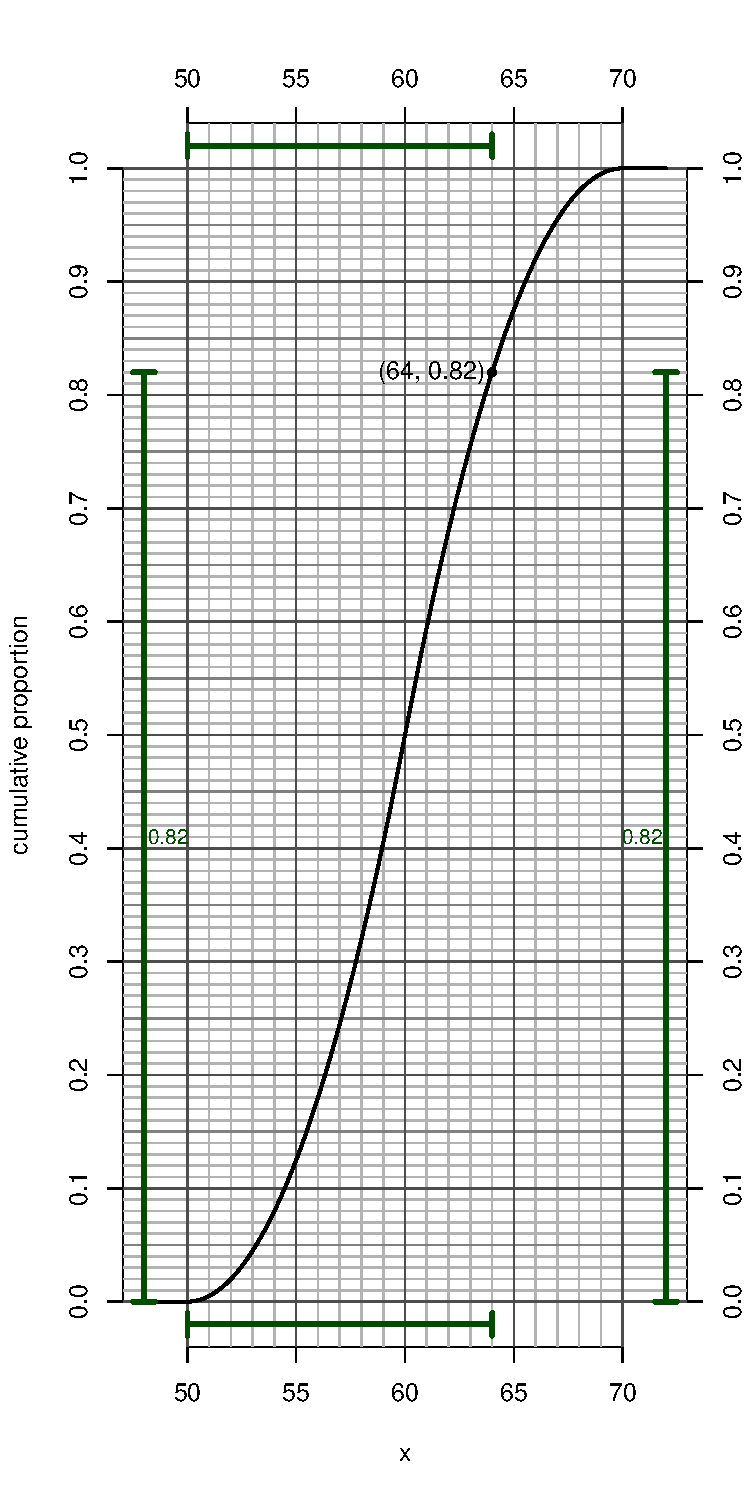
\includegraphics{unnamed-chunk-16-1.pdf} ~
  \item The answer is 56 because \(\text{prop}[\mathbf{x}>56]=0.82\). The
following visualizations show this. The density curve can be used by
counting percent boxes. Each box adds 0.01 to the proportion. You may
need to count half boxes, or find partial boxes that add to whole boxes.
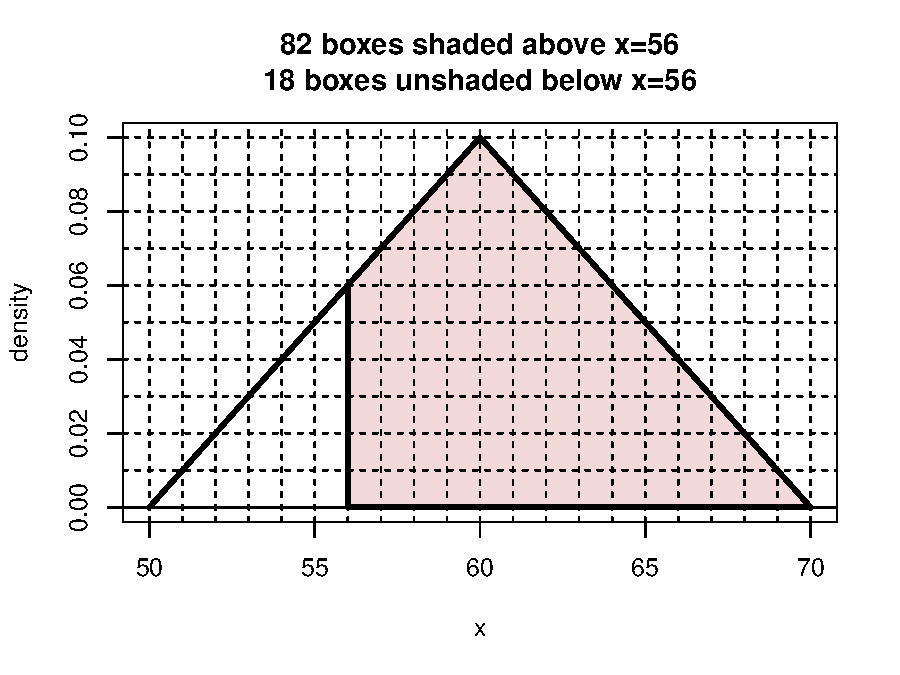
\includegraphics{unnamed-chunk-17-1.pdf} ~ On the spinner, you can
determine the size of a region by using the outside tickmarks.
\[1-0.18=0.82\] 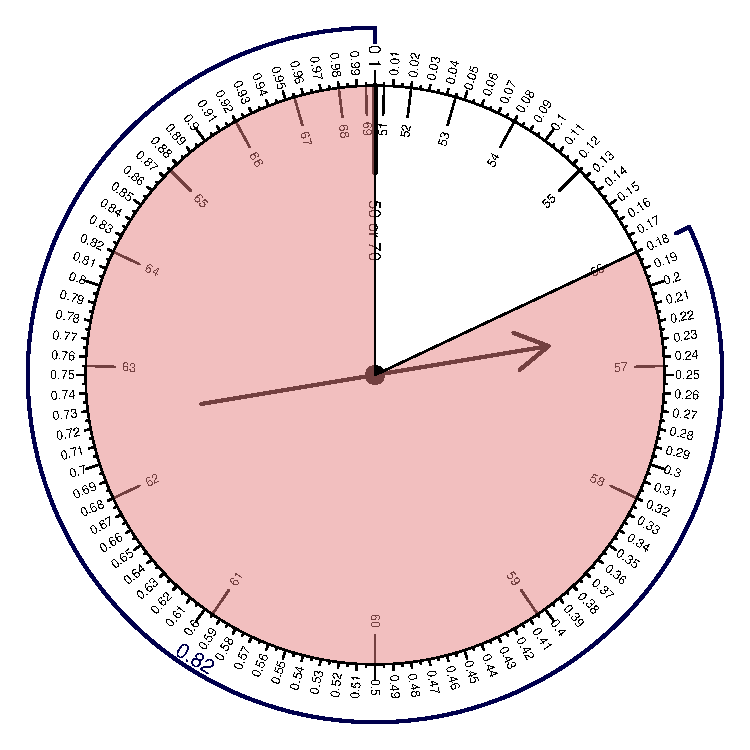
\includegraphics{unnamed-chunk-18-1.pdf} ~ You need to
read coordinates to use the cumulative curve. \[1-0.18=0.82\]
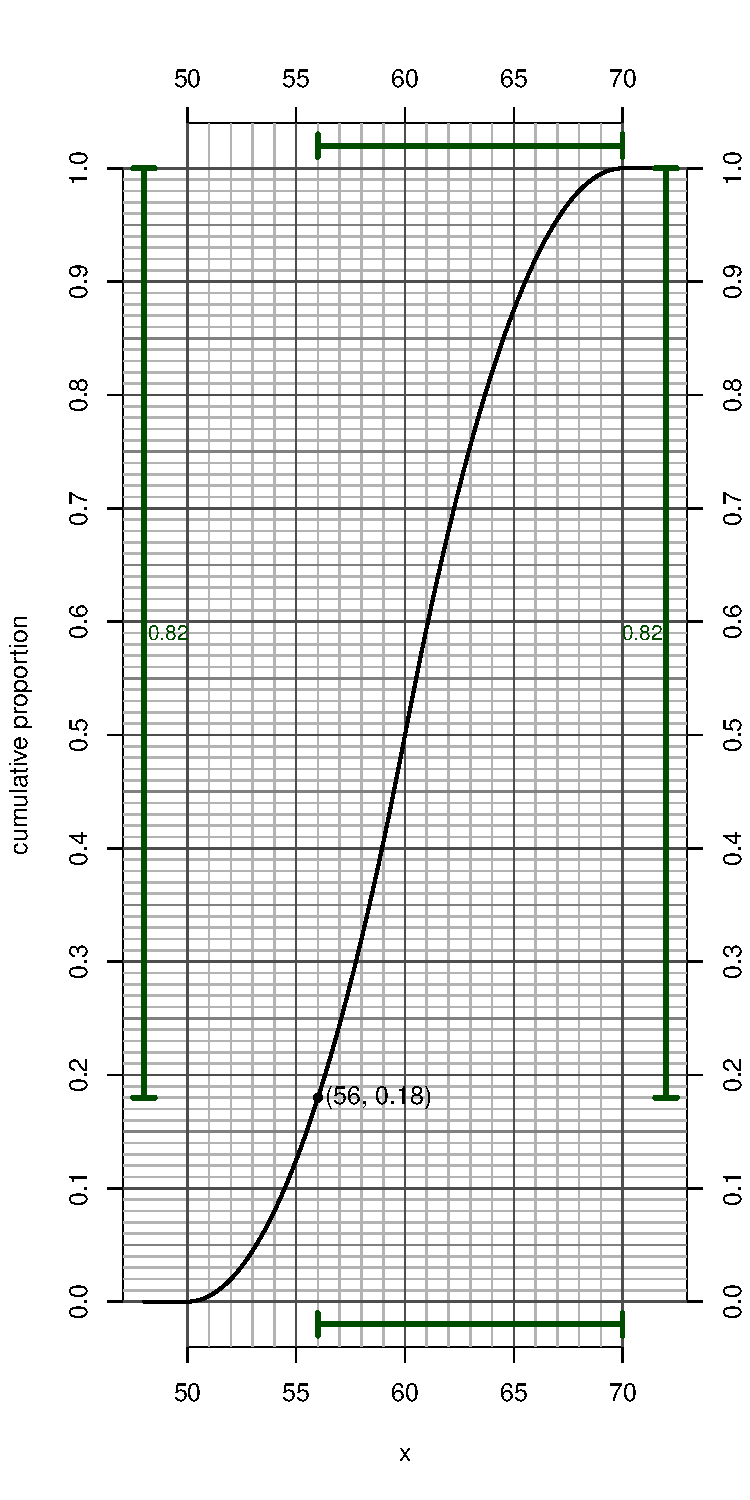
\includegraphics{unnamed-chunk-19-1.pdf} ~
  \item The answer is 3 because \(\text{prop}[|\mathbf{x}-63|<3]=0.42\). You
will need to guess and check to arrive at this answer. The following
shows how to check after making the correct guess. This interval has a
center of 63 and a radius of 3, and thus a lower bound of 60 and an
upper bound of 66. The density curve can be used by counting percent
boxes. Each box adds 0.01 to the proportion. You may need to count half
boxes, or find partial boxes that add to whole boxes.
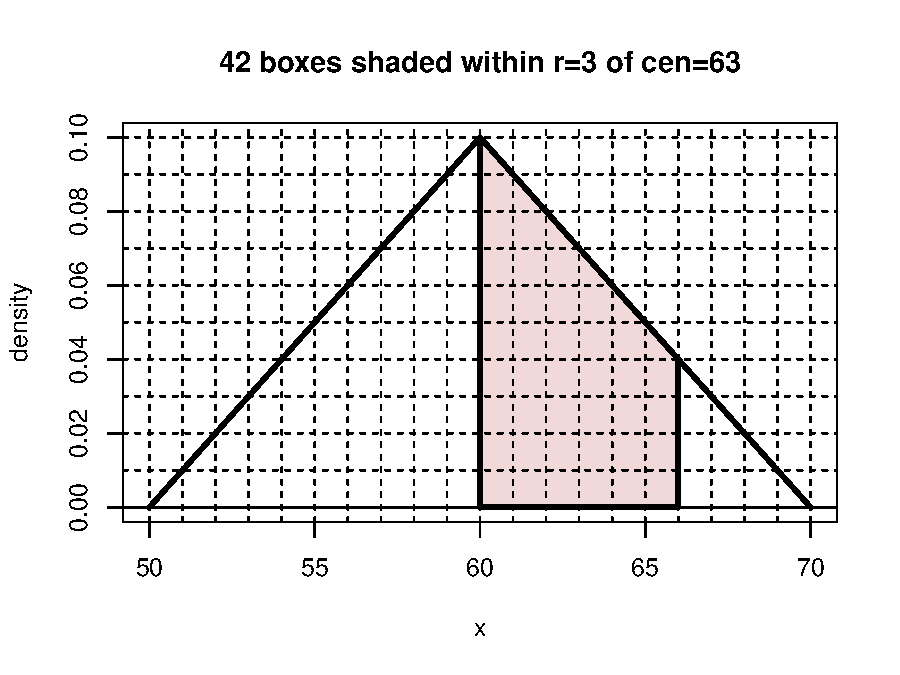
\includegraphics{unnamed-chunk-20-1.pdf} ~ On the spinner, you can
determine the size of a region by using the outside tickmarks. The lower
bound is at \(x=60\), which corresponds to a cumulative proportion of
0.5. The upper bound is at \(x=66\), which corresponds to a cumulative
proportion of 0.92. \[0.92-0.5=0.42\]
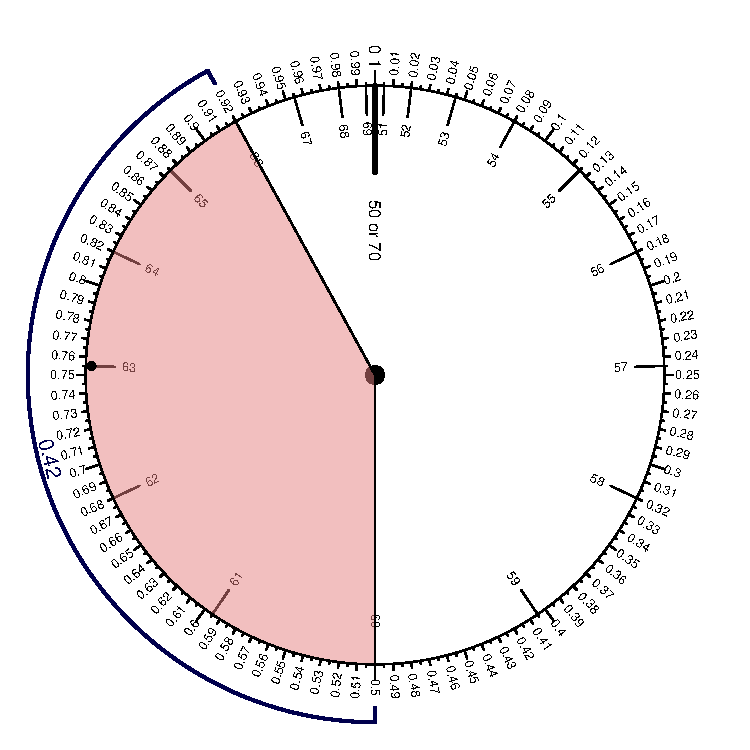
\includegraphics{unnamed-chunk-21-1.pdf} ~ You need to read coordinates
to use the cumulative curve. The lower bound is at \(x=60\), which
corresponds to a cumulative proportion of 0.5. The upper bound is at
\(x=66\), which corresponds to a cumulative proportion of 0.92.
\[0.92-0.5=0.42\] 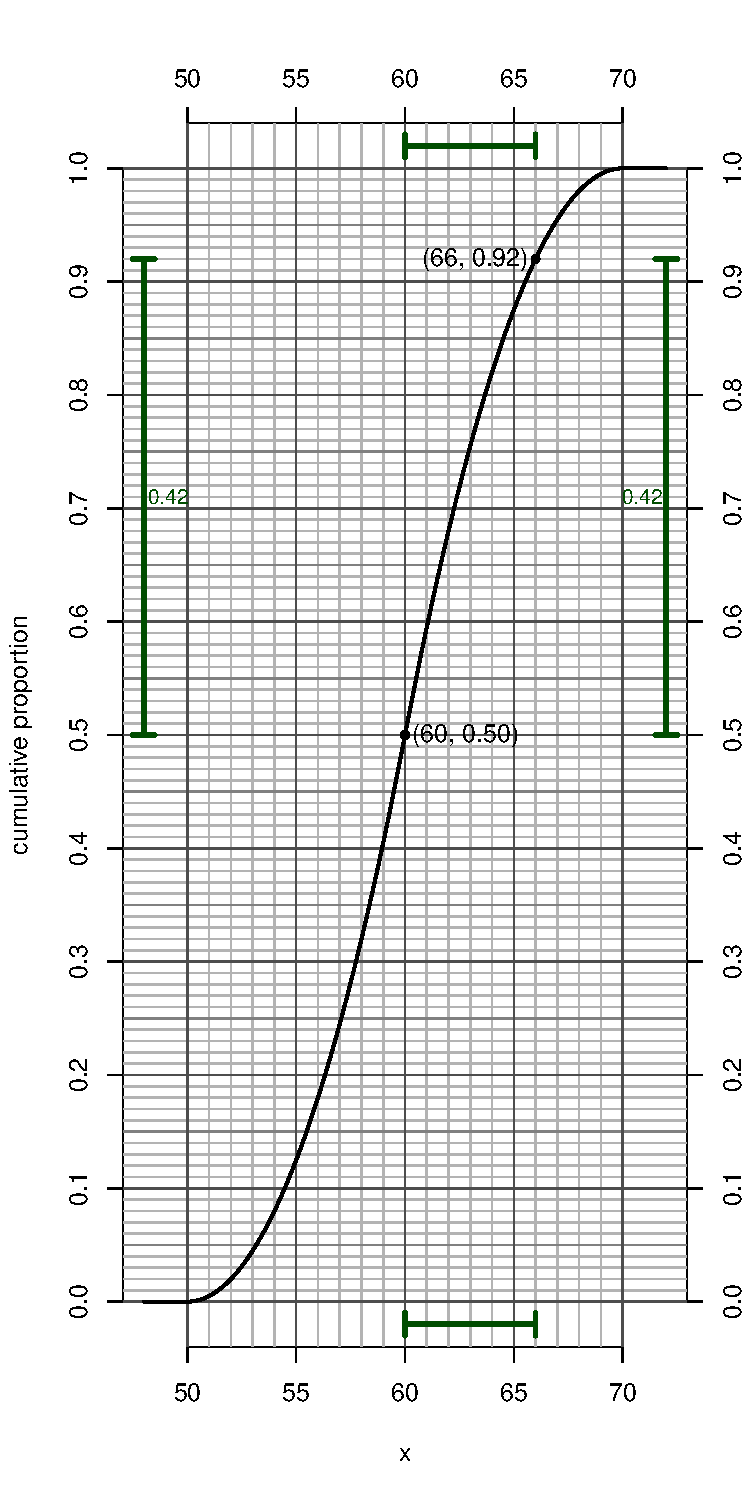
\includegraphics{unnamed-chunk-22-1.pdf}\\
\end{answerlist}
\end{solution}


\end{enumerate}
\end{document}
